\section{Temporal-Aware GRPO for Long-Horizon Policy Optimization}
\label{sec:ta_grpo}

CPT and SFT provide cross-game control and task-following capabilities, while online RL improves the policy on states encountered during its own interactions. Online RL in real-time games faces two challenges: long interactions can exceed the model's context window, and delayed model responses can change the environment transitions observed during rollout collection. We address the first using Temporal-Aware GRPO (TA-GRPO) and the second using the shared Streaming-vLLM infrastructure (Sec.~\ref{sec:streaming_vllm}). Together, they enable policy optimization over long sequences of real-time keyboard and mouse interaction.

As illustrated in Figure~\ref{fig:ta_grpo}, TA-GRPO divides long rollouts into finite segments linked by the same memory compaction mechanism used during SFT. It scores segments from separate rollouts of the same task using verifiable outcomes and assigns group-relative advantages~\cite{shao2024deepseekmath} to the decisions within each segment. The policy can therefore learn from long interactions without fitting a full trajectory into one context or repeatedly restoring an intermediate game state. The policy retains the same input and output format, generating reasoning, memory updates, and executable actions as needed.

\begin{figure*}[!t]
    \centering
    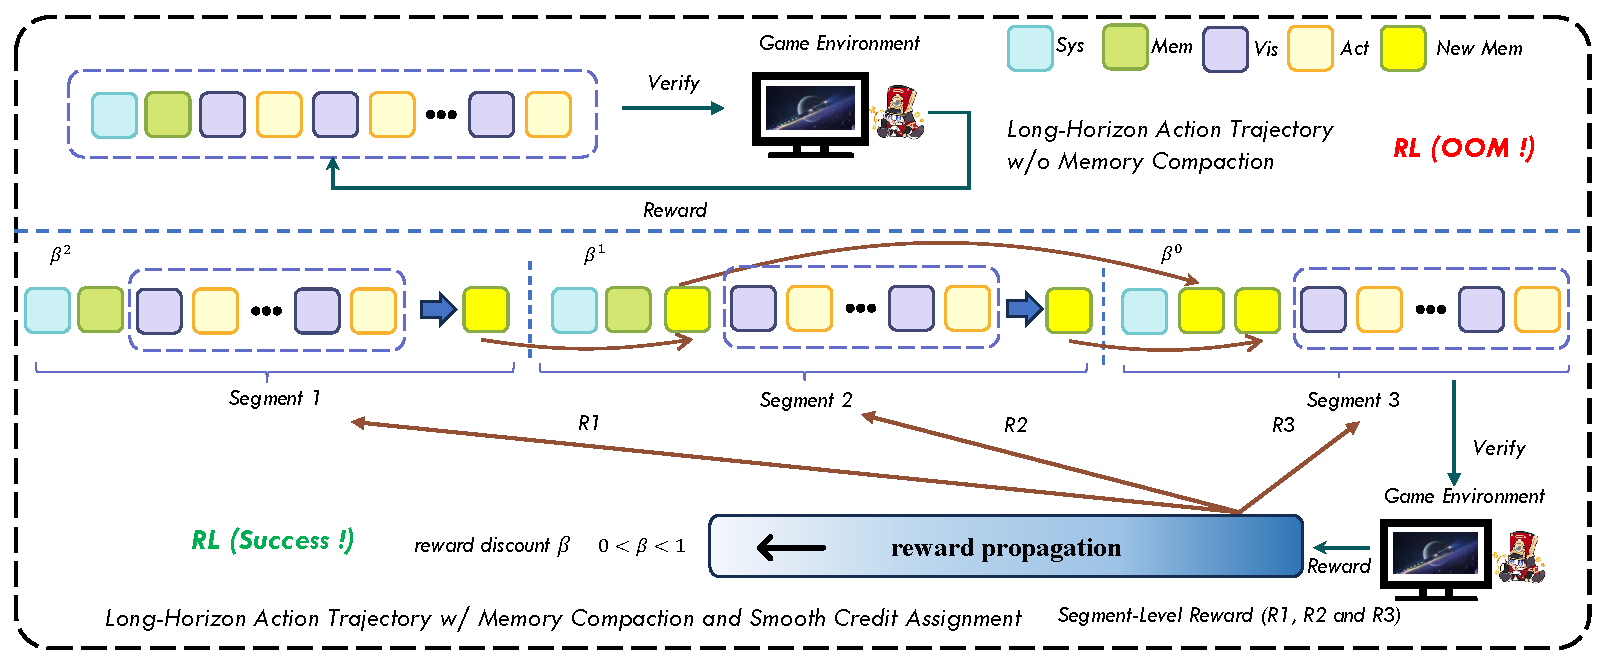
\includegraphics[width=0.89\linewidth]{figs/ta_grpo.pdf}
    \caption{\textbf{Memory-linked long-horizon optimization with TA-GRPO}. A long interaction may exceed the model's context budget (top). Memory compaction divides online rollouts into finite segments whose task states remain connected by generated summaries (bottom). Segments at corresponding stages are compared using environment-verifiable outcomes, and temporal credit assignment distributes their group-relative advantage across decisions. The figure is schematic, and model execution uses the real-time serving backend in Sec.~\ref{sec:streaming_vllm}.}
    \label{fig:ta_grpo}
\end{figure*}

\subsection{Memory-Linked Rollouts}
\label{sec:ta_grpo_segments}

For a task instruction $I$, the old policy $\pi_{\theta_{\mathrm{old}}}$ samples $G$ long-horizon rollouts from the same task condition. Memory compaction partitions rollout $g$ into $J_g$ consecutive segments $\tau_{g,1},\ldots,\tau_{g,J_g}$, each containing $T_{g,m}$ interaction steps. At step $t$ of segment $m$, the policy receives $x_{g,m,t}=(\mathcal B,I,\mathcal M_{g,m,t},\mathcal H_{g,m,t})$ and generates $y_{g,m,t}=(r_{g,m,t},a_{g,m,t})$. The memory produced at a segment boundary carries completed objectives, failures, and remaining plans into subsequent segments. Earlier detailed observations may leave the active context without resetting the task.

For each segment index $m$, we form a comparison group from rollouts that reach that stage, with index set $\mathcal V_m$ and size $G_m=|\mathcal V_m|$. Unlike state-level branching, these segments are not required to start from identical intermediate game states. Grouping rollouts by task condition and compaction stage avoids costly game-state restoration. The shared action format keeps output structure and interaction granularity consistent. This grouping makes computation more regular, although the segments may still differ in difficulty and state distribution. Environment-verifiable feedback determines the relative outcomes used for learning.

\subsection{Verifiable Rewards and Temporal Credit Assignment}
\label{sec:ta_grpo_reward}
\label{sec:temporal_credit}

Long-horizon tasks often expose sparse terminal feedback, although some intermediate objectives admit direct verification. We use the verified outcome $R_{g,m}^{\mathrm{env}}$ of the segment's current objective as its score $S_{g,m}=R_{g,m}^{\mathrm{env}}$. When milestone completion is verifiable, it can provide feedback before the entire quest ends. Otherwise, the score remains sparse. No learned process reward model or value critic is required. Environment-side verification may access task state for training and evaluation, while the deployed policy still observes only the screen and issues keyboard-mouse actions.

Within the group at stage $m$, scores are normalized to obtain a relative segment advantage:
\begin{equation}
\label{eq:segment_advantage}
A_{g,m}=\frac{S_{g,m}-\mu_m}{s_m},\qquad
\mu_m=\frac{1}{G_m}\sum_{g\in\mathcal V_m}S_{g,m},\quad
s_m=\sqrt{\frac{1}{G_m}\sum_{g\in\mathcal V_m}(S_{g,m}-\mu_m)^2+\epsilon_{\mathrm{grp}}}.
\end{equation}
This critic-free estimate follows GRPO~\cite{shao2024deepseekmath}. Because verification typically occurs at a segment boundary, the segment score does not identify the contributions of individual decisions. TA-GRPO assigns larger weights to later steps, which are temporally closer to that outcome, while normalizing the weights to preserve their mean:
\begin{equation}
\label{eq:temporal_advantage}
\widetilde d_{g,m,t}=\frac{\beta^{T_{g,m}-1-t}}{\frac{1}{T_{g,m}}\sum_{u=0}^{T_{g,m}-1}\beta^{T_{g,m}-1-u}},\qquad
A_{g,m,t}=\widetilde d_{g,m,t}A_{g,m},\quad \beta\in(0,1).
\end{equation}
The temporal weights average to one, redistributing the segment-level advantage across steps while preserving the mean. This weighting encodes a temporal prior, and it does not imply that later actions contribute more to the outcome.

\subsection{Joint Reasoning-Action Policy Update}
\label{sec:ta_grpo_update}

TA-GRPO updates the autoregressive policy over the complete output $y_{g,m,t}=(r_{g,m,t},a_{g,m,t})$, where $r_{g,m,t}$ may be empty, contain reasoning for the current decision, or provide a memory summary. The low-level action $a_{g,m,t}$ is always generated. For output token $j$, we define the ratio between the current and old policy, conditioned on the preceding output tokens:
\begin{equation}
\label{eq:token_policy_ratio}
\rho_{g,m,t,j}(\theta)=\frac{\pi_\theta(y_{g,m,t,j}\mid x_{g,m,t},y_{g,m,t,<j})}{\pi_{\theta_{\mathrm{old}}}(y_{g,m,t,j}\mid x_{g,m,t},y_{g,m,t,<j})}.
\end{equation}
We use the standard token-level clipped GRPO surrogate, with $\rho=\rho_{g,m,t,j}(\theta)$ and $A=A_{g,m,t}$ for readability:
\[
\ell_{g,m,t,j}(\theta)
=\min\!\left\{\rho A,\,
\operatorname{clip}\!\left(\rho,1-\epsilon_{\mathrm{clip}},1+\epsilon_{\mathrm{clip}}\right)A\right\}.
\]
The final objective averages this surrogate over valid segments, interaction steps, and output tokens:
\begin{equation}
\label{eq:ta_grpo_objective}
\mathcal L_{\mathrm{TA\text{-}GRPO}}=-\frac{1}{\sum_m G_m}\sum_m\sum_{g\in\mathcal V_m}\frac{1}{T_{g,m}}\sum_{t=0}^{T_{g,m}-1}\frac{1}{|y_{g,m,t}|}\sum_{j=1}^{|y_{g,m,t}|}\ell_{g,m,t,j}(\theta).
\end{equation}
Token-level clipping avoids a single sequence-wide probability ratio whose scale would depend strongly on the combined reasoning and action length. The same learning signal can update memory summaries, sparse reasoning, and executable control. Streaming-vLLM generates these rollouts across concurrent game instances and dispatches actions promptly.
